\documentclass[11pt]{article}
% ---------------------------------------------------------------------------
% _s2_closer in pseudocode, with pictures.
% Compile: module load texlive/2025 && pdflatex closer_pseudocode_handout.tex  (twice)
% Every number is machine-verified (see _closer_viz.py / _trace_closer.py).
% ---------------------------------------------------------------------------
\usepackage[margin=2.0cm]{geometry}
\usepackage{amsmath,amssymb}
\usepackage{xcolor}
\usepackage{tikz}
\usetikzlibrary{positioning,calc,arrows.meta,decorations.pathreplacing,fit,backgrounds}
\usepackage[most]{tcolorbox}
\usepackage{booktabs}
\usepackage{float}
\usepackage{algorithm}
\usepackage{algpseudocode}
\usepackage{parskip}
\usepackage{microtype}

% --- palette ---------------------------------------------------------------
\definecolor{headc}{HTML}{1B7F3B}   % head / green
\definecolor{compc}{HTML}{1F5FBF}   % comp / blue
\definecolor{flipc}{HTML}{C0392B}   % flip / red
\definecolor{invc}{HTML}{555555}    % gray
\definecolor{panel}{HTML}{F4F1EA}
\definecolor{codebg}{HTML}{F7F7F4}

\newcommand{\head}[1]{\textcolor{headc}{#1}}
\newcommand{\comp}[1]{\textcolor{compc}{#1}}
\newcommand{\flip}[1]{\textcolor{flipc}{#1}}
\newcommand{\code}[1]{\texttt{#1}}

\newtcolorbox{rulebox}[1][]{colback=panel,colframe=black!70,boxrule=0.6pt,
  arc=2pt,left=6pt,right=6pt,top=4pt,bottom=4pt,title={#1},fonttitle=\bfseries}
\newtcolorbox{keybox}[1][]{colback=flipc!6,colframe=flipc!75,boxrule=0.8pt,
  arc=2pt,left=6pt,right=6pt,top=4pt,bottom=4pt,title={#1},fonttitle=\bfseries}

% --- pseudocode style ------------------------------------------------------
\algrenewcommand\algorithmicrequire{\textbf{Input:}}
\algrenewcommand\algorithmicensure{\textbf{Output:}}
\algnewcommand\algorithmicand{\textbf{and}}
\newcommand{\sop}[1]{\ensuremath{\mathsf{#1}}}

% --- token-flow diagram (HI row over HF row with permutation arcs) ---------
\newcommand{\tokflow}[4]{%
\begin{tikzpicture}[
   tok/.style={draw=black!55, fill=white, rounded corners=1.5pt,
               minimum height=6.5mm, inner xsep=3pt, font=\footnotesize},
   every node/.style={anchor=center}]
  \def\dx{#1}
  \foreach \i/\lab in {#2}{ \node[tok] (hi\i) at (\i*\dx,2.3) {\lab}; }
  \foreach \m/\lab in {#3}{ \node[tok] (hf\m) at (\m*\dx,0) {\lab}; }
  \node[font=\scriptsize\bfseries, text=invc] at (-1.05,2.3) {HI};
  \node[font=\scriptsize\bfseries, text=invc] at (-1.05,0)   {HF};
  \foreach \a/\b/\c/\t in {#4}{
     \draw[\c, line width=1.1pt, -{Stealth[length=4pt]}, opacity=0.9]
        (hi\a.south) to[out=-90,in=90] node[midway, sloped, above=-1pt,
        font=\tiny, text=\c]{\t} (hf\b.north);
  }
\end{tikzpicture}}

% --- a row of cells (an s-op) ---------------------------------------------
% \soprow{yshift}{label}{v0,...,v6}{fillcolor}
\newcommand{\cellrow}[4]{%
  \node[font=\scriptsize\ttfamily, text=invc, anchor=east] at (-0.55,#1) {#2};
  \foreach \v [count=\i from 0] in {#3}{
     \node[draw=black!45, fill=#4, minimum size=6.2mm, inner sep=0pt,
           font=\scriptsize] at (\i,#1) {\v};}}

\begin{document}

\begin{center}
  {\LARGE\bfseries \texttt{\_s2\_closer}, in Pseudocode}\\[3pt]
  {\large every stage as an algorithm, every algorithm as a picture}\\[5pt]
  {\small Running example:}\\[1pt]
  {\small\ttfamily HI = the boy that chases the dog swims}\\[1pt]
  {\small\ttfamily HF = the the dog chases that boy swims}
\end{center}
\vspace{4pt}\hrule\vspace{6pt}

% ==========================================================================
\section{Notation: what the program manipulates}

Everything is an \textbf{s-op}: a length-$n$ array holding \emph{one value per token position}.
Positions are $0,\dots,n-1$. Nothing else exists --- no stack, no tree, no recursion.

\begin{center}
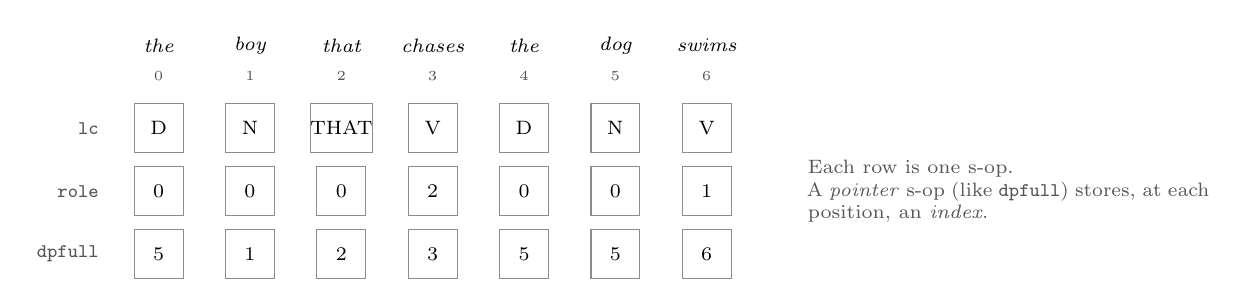
\begin{tikzpicture}[xscale=1.16, font=\footnotesize]
  \foreach \w [count=\i from 0] in {the,boy,that,chases,the,dog,swims}{
    \node[font=\scriptsize\itshape] at (\i,1.05) {\w};
    \node[font=\tiny, text=invc] at (\i,0.66) {\i};}
  \cellrow{0}{lc}{D,N,THAT,V,D,N,V}{white}
  \cellrow{-0.8}{role}{0,0,0,2,0,0,1}{white}
  \cellrow{-1.6}{dpfull}{5,1,2,3,5,5,6}{white}
  \node[anchor=west, font=\scriptsize, text=invc] at (7.0,-0.8)
    {\begin{minipage}{5.1cm}Each row is one s-op.\\ A \emph{pointer} s-op (like \code{dpfull}) stores, at each position, an \emph{index}.\end{minipage}};
\end{tikzpicture}
\end{center}

\subsection{The four primitives}
Every line of the program is one of these. Only the last three move information between positions.

\begin{center}\footnotesize
\begin{tabular}{@{}llp{7.6cm}@{}}
\toprule
primitive & meaning & cost\\
\midrule
$\textsc{Map}(x,f)$, $\textsc{Where}(c,a,b)$ & elementwise & an MLP (free, no communication)\\
$\textsc{Read}(x,\delta)$ & $\text{out}[i]=x[i{+}\delta]$ & 1 attention head (relative offset)\\
$\textsc{Gather}(x,p)$ & $\text{out}[i]=x[\,p[i]\,]$ & 1 attention head (pointer chase)\\
$\textsc{Stab}(\mathit{ends})$ & $\#\{j\le i: \mathit{ends}[j]\ge i\}$ & 1 counting head\\
\bottomrule
\end{tabular}
\end{center}

\begin{keybox}[The naming convention you must internalize]
\code{A\_at\_B} $\;=\;\textsc{Gather}(\code{A},\code{B})$, i.e. \;$\code{A\_at\_B}[i] = \code{A}\big[\code{B}[i]\big]$.\\[3pt]
Read it as ``\emph{the value of \code{A}, fetched from the position named by \code{B}, delivered to $i$}.''
The suffix names \emph{where the value came from}. This is how a token reaches a distant
constituent without ever using an absolute index: it computes \emph{where} the thing it needs
\emph{starts}, then gathers that thing's end-pointer from there.
\end{keybox}

\paragraph{Picture of \textsc{Gather}.} Take \code{dpfull\_at\_hb1} $=\textsc{Gather}(\code{dpfull},\code{hb1})$
at the verb \emph{chases}$_3$. Its complement starts at $\code{hb1}[3]=4$; we go read \code{dpfull} there and bring $5$ back.

\begin{center}
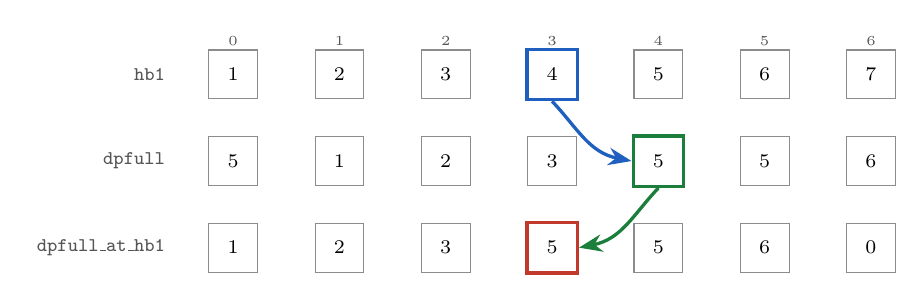
\begin{tikzpicture}[xscale=1.35, font=\footnotesize]
  \foreach \i in {0,...,6} \node[font=\tiny, text=invc] at (\i,2.62) {\i};
  \cellrow{2.2}{hb1}{1,2,3,4,5,6,7}{white}
  \cellrow{1.1}{dpfull}{5,1,2,3,5,5,6}{white}
  \cellrow{0.0}{dpfull\_at\_hb1}{1,2,3,5,5,6,0}{white}
  \node[draw=compc, very thick, minimum size=6.4mm, inner sep=0pt] (h3) at (3,2.2) {};
  \node[draw=headc, very thick, minimum size=6.4mm, inner sep=0pt] (d4) at (4,1.1) {};
  \node[draw=flipc, very thick, minimum size=6.4mm, inner sep=0pt] (o3) at (3,0.0) {};
  \draw[compc,-{Stealth},very thick] (h3.south) to[out=-55,in=165] (d4.west);
  \draw[headc,-{Stealth},very thick] (d4.south) to[out=-125,in=15]  (o3.east);
\end{tikzpicture}
\end{center}
\vspace{-4pt}
\noindent{\footnotesize \textcolor{compc}{\textbf{Blue}}: $\code{hb1}[3]=4$ says \emph{where to look}.\;
\textcolor{headc}{\textbf{Green}}: $\code{dpfull}[4]=5$ is the value carried back into
$\code{dpfull\_at\_hb1}[3]$. So \emph{chases}$_3$ learns ``my complement starts at 4, and it ends at 5''.}

% ==========================================================================
\section{Top level}

HF is a \emph{permutation} of HI, so the program never generates: it computes a target slot per
token and gathers.

\begin{algorithm}[H]
\caption{\textsc{HiToHf}$(w[0..n{-}1])$ --- head-initial $\to$ head-final}
\begin{algorithmic}[1]
\Require surface words $w$
\Ensure the head-final reordering
\State $\sop{ids} \gets \textsc{Map}(w,\ \text{WORD2ID})$ \Comment{token embedding}
\State $\sop{i} \gets [\,0,1,\dots,n-1\,]$ \Comment{position s-op}
\State $(\sop{lc},\sop{role},\sop{isThat},\sop{isCrel},\sop{isC}) \gets \textsc{Stage1}(\sop{ids})$ \Comment{local, \S3}
\State $(\sop{hbEnd},\sop{dpFlat},\sop{rcPos},\sop{hasRC}) \gets \textsc{Scaffold}(\dots)$ \Comment{one-shot, \S4}
\State $(\sop{dpfull},\sop{vpe},\sop{rce},\sop{cpe}) \gets \textsc{Relax}(\dots)$ \Comment{the loop, \S5}
\State $\sop{e} \gets \textsc{Where}(\sop{isCrel},\ \sop{rce},\ \textsc{Where}(\sop{isC},\ \sop{cpe},\ \sop{i}))$ \Comment{clause end per opener}
\State $\sop{depth} \gets \textsc{Stab}\big(\textsc{Where}(\sop{isThat},\ \sop{e},\ -1)\big)$ \Comment{nesting depth}
\State $\sop{disp} \gets \sop{d\_adv}+\sop{d\_cp}+\sop{d\_nprel}+\sop{d\_vp}$ \Comment{\S6}
\State $\sop{hfPos} \gets \sop{i} + \sop{disp}$ \Comment{target slot of each token}
\State $\sop{src} \gets \textsc{Invert}(\sop{hfPos})$ \Comment{\S7}
\State \Return $\textsc{Decode}\big(\textsc{Gather}(\sop{ids},\ \sop{src})\big)$
\end{algorithmic}
\end{algorithm}

\noindent Only line 5 is hard. Lines 1--4 are local; lines 6--11 are counting and one gather.

% ==========================================================================
\section{Stage 1 --- local part of speech and verb role}

\begin{algorithm}[H]
\caption{\textsc{Stage1} --- everything from a token and its neighbours}
\begin{algorithmic}[1]
\State $\sop{lc} \gets \textsc{Map}(\sop{ids},\ \textsc{LexClass})$ \Comment{$\in\{$D, N, Nprop, Adj, Adv, THAT, V$\}$}
\State $\sop{prev},\sop{prev2} \gets \textsc{Read}(\sop{lc},-1),\ \textsc{Read}(\sop{lc},-2)$
\State $\sop{next},\sop{next2} \gets \textsc{Read}(\sop{lc},+1),\ \textsc{Read}(\sop{lc},+2)$
\State $\sop{isThat} \gets [\,\sop{lc}=\text{THAT}\,]$ \Comment{the clause \emph{openers}}
\State $\sop{isCrel} \gets \sop{isThat} \wedge [\,\sop{prev}=\text{N}\,]$ \Comment{\emph{that} after a common noun $\Rightarrow$ relative}
\State $\sop{isC} \gets \sop{isThat} \wedge \lnot\,\sop{isCrel}$ \Comment{otherwise sentential}
\State $\sop{nn} \gets \textsc{Where}\big([\,\sop{next}=\text{Adv}\,],\ \sop{next2},\ \sop{next}\big)$ \Comment{next \emph{non-adverb} class}
\If{$\lnot\,[\,\sop{lc}=\text{V}\,]$} \State $\sop{role}\gets 0$ \Comment{not a verb}
\ElsIf{$[\,\sop{nn}=\text{THAT}\,]$} \State $\sop{role}\gets 3$ \Comment{$+$clause \;(\code{V\_cp})}
\ElsIf{$[\,\sop{nn}\in\{\text{D},\text{Nprop}\}\,]$} \State $\sop{role}\gets 2$ \Comment{$+$object DP \;(\code{V\_dp})}
\ElsIf{$\sop{isIntrans}$} \State $\sop{role}\gets 1$ \Comment{intransitive}
\Else \State $\sop{role}\gets 4$ \Comment{object-gap (transitive verb, no object)}
\EndIf
\end{algorithmic}
\end{algorithm}

\begin{rulebox}[Why \sop{role} is the whole point]
Roles \head{2} and \head{3} are the verbs that \flip{flip} (they have a complement to reverse with);
roles \comp{1} and \comp{4} never flip. One forward neighbour read decides it.
\end{rulebox}

\noindent On the running example (all values machine-verified):
\begin{center}\footnotesize
\begin{tabular}{@{}l|ccccccc@{}}
\toprule
 & the$_0$ & boy$_1$ & that$_2$ & chases$_3$ & the$_4$ & dog$_5$ & swims$_6$\\
\midrule
\code{lc}      & D & N & THAT & V & D & N & V\\
\code{isThat}  & 0 & 0 & 1 & 0 & 0 & 0 & 0\\
\code{isCrel}  & 0 & 0 & \flip{1} & 0 & 0 & 0 & 0\\
\code{role}    & 0 & 0 & 0 & \head{2} & 0 & 0 & \comp{1}\\
\bottomrule
\end{tabular}
\end{center}

% ==========================================================================
\section{Stage 2a --- one-shot scaffolding}

Three fixed-offset facts, computed once, \emph{before} any iteration.

\begin{algorithm}[H]
\caption{\textsc{Scaffold} --- local span pieces}
\begin{algorithmic}[1]
\State $\sop{hbEnd} \gets \textsc{Where}\big([\,\sop{lc}{=}\text{V}\,]\wedge[\,\sop{next}{=}\text{Adv}\,],\ \sop{i}{+}1,\ \sop{i}\big)$ \Comment{verb\,(+adverb) head block}
\State $\sop{dpFlat} \gets \textsc{Where}\big([\,\sop{lc}{=}\text{D}\,],\ \textsc{Where}([\,\sop{next}{=}\text{Adj}\,],\ \sop{i}{+}2,\ \sop{i}{+}1),\ \sop{i}\big)$ \Comment{DP end \emph{ignoring} a rel.\ clause}
\State $\sop{rcPos} \gets \sop{dpFlat}+1$ \Comment{slot where a relative \emph{that} would sit}
\State $\sop{hasRC} \gets [\,\sop{lc}{=}\text{D}\,]\ \wedge\ [\,\textsc{Gather}(\sop{lc},\sop{rcPos})=\text{THAT}\,]$ \Comment{one lookahead}
\end{algorithmic}
\end{algorithm}

\paragraph{\code{dpFlat} by example.} \emph{the nice boy} $\Rightarrow$ \code{dpFlat}$=[2,1,2]$: the determiner
steps over the adjective ($i{+}2$); the other cells are the harmless $\sop{i}$ filler.
\emph{the boy} $\Rightarrow [1,1]$.

\paragraph{\code{hasRC} by example.} At \emph{the}$_0$: $\code{rcPos}[0]=\code{dpFlat}[0]{+}1=2$, and
$\code{lc}[2]=\text{THAT}$ $\Rightarrow$ \code{hasRC}$[0]=1$. That DP carries a relative clause.

% ==========================================================================
\section{Stage 2b --- \textsc{Relax}: the heart}

\subsection{What we are trying to build}
Four \textbf{end pointers}, each keyed by \emph{start} position: $\code{ptr}[i]$ = last index of the
constituent of that type that \emph{begins} at $i$.

\begin{center}
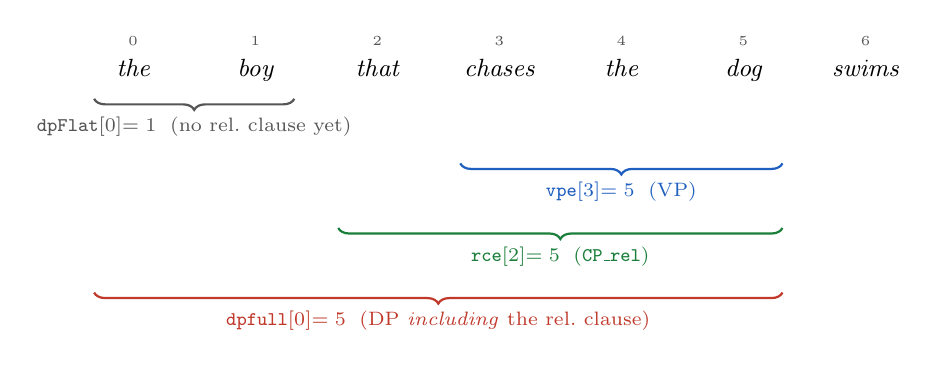
\begin{tikzpicture}[xscale=1.55, font=\footnotesize]
 \foreach \w [count=\i from 0] in {the,boy,that,chases,the,dog,swims}{
   \node[anchor=base, font=\small\itshape] at (\i,0) {\w};
   \node[font=\tiny, text=invc] at (\i,0.45) {\i};}
 \draw[decorate,decoration={brace,amplitude=4pt,mirror},invc,thick] (-0.32,-0.28)--(1.32,-0.28)
   node[midway,below=3pt,font=\scriptsize,text=invc]{\code{dpFlat}[0]$=1$ \;(no rel.\ clause yet)};
 \draw[decorate,decoration={brace,amplitude=4pt,mirror},compc,thick] (2.68,-1.10)--(5.32,-1.10)
   node[midway,below=3pt,font=\scriptsize,text=compc]{\code{vpe}[3]$=5$ \;(VP)};
 \draw[decorate,decoration={brace,amplitude=4pt,mirror},headc,thick] (1.68,-1.92)--(5.32,-1.92)
   node[midway,below=3pt,font=\scriptsize,text=headc]{\code{rce}[2]$=5$ \;(\code{CP\_rel})};
 \draw[decorate,decoration={brace,amplitude=4pt,mirror},flipc,thick] (-0.32,-2.74)--(5.32,-2.74)
   node[midway,below=3pt,font=\scriptsize,text=flipc]{\code{dpfull}[0]$=5$ \;(DP \emph{including} the rel.\ clause)};
\end{tikzpicture}
\end{center}

\noindent They are \textbf{mutually recursive} --- each needs another's answer:
\[
 \underbrace{\code{dpfull}}_{\text{DP}}\ \longrightarrow\ \underbrace{\code{rce}}_{\text{CP\_rel}}\ \longrightarrow\ \underbrace{\code{vpe}}_{\text{VP}}\ \longrightarrow\ \underbrace{\code{cpe}}_{\text{CP\_sent}}\ \longrightarrow\ \code{vpe}\ \longrightarrow \cdots
\]
so no single pass can compute them. We \emph{relax}: seed a lower bound, re-apply the rules until nothing changes.

\begin{algorithm}[H]
\caption{\textsc{Relax}$(K)$ --- resolve the mutually recursive END pointers}
\begin{algorithmic}[1]
\State $\sop{dpfull}\gets\sop{dpFlat};\quad \sop{vpe}\gets\sop{hbEnd};\quad \sop{rce}\gets\sop{i};\quad \sop{cpe}\gets\sop{i}$ \Comment{seed: ``each ends at itself''}
\For{$r = 1$ \textbf{to} $K$} \Comment{one sweep $=$ one attention hop $=$ one nesting level}
  \State $\sop{dpfull}\gets\textsc{Where}\big(\sop{hasRC},\ \textsc{Gather}(\sop{rce},\sop{rcPos}),\ \sop{dpFlat}\big)$ \Comment{extend over the rel.\ clause}
  \State \Comment{a VP ends where its complement ends; the complement starts at $\sop{hbEnd}{+}1$}
  \If{$\sop{role}\in\{1,4\}$} \State $\sop{vpe}\gets\sop{hbEnd}$ \Comment{no complement}
  \ElsIf{$\sop{role}=2$} \State $\sop{vpe}\gets\textsc{Gather}(\sop{dpfull},\ \sop{hbEnd}{+}1)$ \Comment{object DP's end}
  \ElsIf{$\sop{role}=3$} \State $\sop{vpe}\gets\textsc{Gather}(\sop{cpe},\ \sop{hbEnd}{+}1)$ \Comment{embedded clause's end}
  \EndIf
  \State \Comment{a relative clause ends where its gap-clause ends}
  \If{$\sop{isCrel}$ \algorithmicand\ $[\,\sop{next}=\text{V}\,]$} \State $\sop{rce}\gets\textsc{Gather}(\sop{vpe},\ \sop{i}{+}1)$ \Comment{subject gap: it \emph{is} a VP}
  \ElsIf{$\sop{isCrel}$} \State $\sop{rce}\gets\textsc{Gather}(\sop{dpfull},\ \sop{i}{+}1)+1$ \Comment{object gap: the gap verb}
  \EndIf
  \State $\sop{vpos}\gets\textsc{Gather}(\sop{dpfull},\ \sop{i}{+}1)+1$ \Comment{embedded VP starts past the subject DP}
  \State $\sop{cpe}\gets\textsc{Where}\big(\sop{isC},\ \textsc{Gather}(\sop{vpe},\ \sop{vpos}),\ \sop{i}\big)$
\EndFor
\end{algorithmic}
\end{algorithm}

\begin{keybox}[Loop invariant]
After $r$ sweeps, \textbf{every constituent with fewer than $r$ levels of nesting beneath it has its
exact end}. Each \textsc{Gather} follows exactly \emph{one} pointer, so one sweep advances the
``resolved frontier'' by exactly one level, from the inside out. Hence
$\;\text{sweeps needed}\;\approx\;\text{nesting depth}$, and \code{ROUNDS} is the program's
\emph{depth budget}.
\end{keybox}

\subsection{The ripple, depth 1}
For our sentence the chain is $\code{dpFlat}[4]\!\to\!\code{vpe}[3]\!\to\!\code{rce}[2]\!\to\!\code{dpfull}[0]$.
Because \code{dpfull} is updated \emph{before} \code{rce} in each sweep, it lags one sweep behind:

\begin{center}\footnotesize
\begin{tabular}{@{}l|ccc|l@{}}
\toprule
 & \code{vpe}[3] & \code{rce}[2] & \code{dpfull}[0] & \\
\midrule
seed   & 3 & 2 & 1 & ``each ends at itself'' / flat\\
sweep 1 & \head{5} & \head{5} & \flip{2} & \code{dpfull} read a \emph{stale} \code{rce}\\
sweep 2 & 5 & 5 & \head{5} & now correct\\
sweep 3--10 & 5 & 5 & 5 & fixed point (nothing changes)\\
\bottomrule
\end{tabular}
\end{center}

\subsection{The ripple, depth 2 --- why layers scale with depth}
\emph{John knows that Mary knows that the dog swims}: both clauses close on \emph{swims}$_8$.

\begin{center}\footnotesize
\begin{tabular}{@{}l|cc|l@{}}
\toprule
 & \code{cpe}[5] (inner) & \code{cpe}[2] (outer) & \\
\midrule
seed    & 5 & 2 & \\
sweep 1 & \head{8} & \flip{5} & inner bottoms out at once; outer stops one level short\\
sweep 2 & 8 & \head{8} & outer inherits the inner clause's end\\
\bottomrule
\end{tabular}
\end{center}

\begin{center}
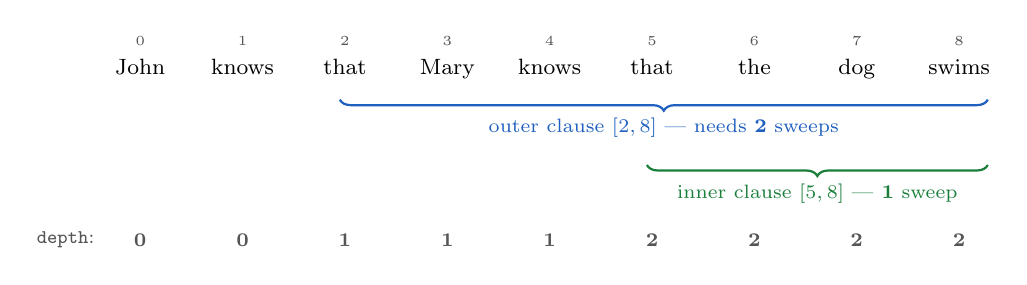
\begin{tikzpicture}[font=\footnotesize, xscale=1.30]
  \foreach \w [count=\i from 0] in {John,knows,that,Mary,knows,that,the,dog,swims}{
     \node[anchor=base] at (\i,0) {\w};
     \node[font=\tiny,text=invc] at (\i,0.42) {\i};}
  \draw[compc,thick,decorate,decoration={brace,amplitude=4pt,mirror}]
     (1.95,-0.32)--(8.28,-0.32) node[midway,below=3pt,font=\scriptsize,text=compc]{outer clause $[2,8]$ --- needs \textbf{2} sweeps};
  \draw[headc,thick,decorate,decoration={brace,amplitude=4pt,mirror}]
     (4.95,-1.15)--(8.28,-1.15) node[midway,below=3pt,font=\scriptsize,text=headc]{inner clause $[5,8]$ --- \textbf{1} sweep};
  \foreach \i/\d in {0/0,1/0,2/1,3/1,4/1,5/2,6/2,7/2,8/2}
     \node[font=\scriptsize\bfseries,text=invc] at (\i,-2.1) {\d};
  \node[font=\scriptsize,text=invc,anchor=east] at (-0.35,-2.1) {\code{depth}:};
\end{tikzpicture}
\end{center}

% ==========================================================================
\section{Stage 2c --- depth, then displacement}

\subsection{\textsc{Stab}: turn intervals into a count}
Each opener now owns an interval $[q,\ e(q)]$. \code{depth}$[i]$ counts how many cover $i$ --- one head.

\begin{center}
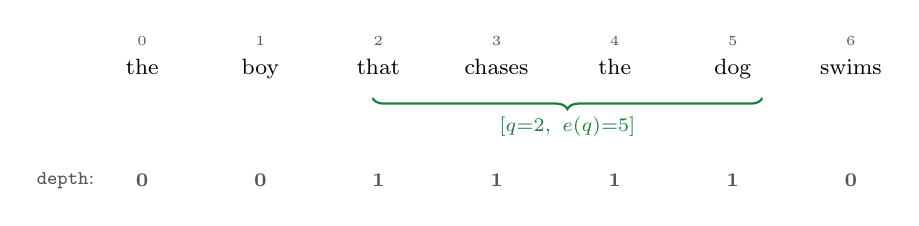
\begin{tikzpicture}[font=\footnotesize, xscale=1.5]
  \foreach \w [count=\i from 0] in {the,boy,that,chases,the,dog,swims}{
    \node[anchor=base] at (\i,0) {\w};
    \node[font=\tiny,text=invc] at (\i,0.42) {\i};}
  \draw[headc,thick,decorate,decoration={brace,amplitude=4pt,mirror}]
    (1.95,-0.3)--(5.25,-0.3) node[midway,below=3pt,font=\scriptsize,text=headc]{$[q{=}2,\ e(q){=}5]$};
  \foreach \i/\d in {0/0,1/0,2/1,3/1,4/1,5/1,6/0}
    \node[font=\scriptsize\bfseries,text=invc] at (\i,-1.35) {\d};
  \node[font=\scriptsize,text=invc,anchor=east] at (-0.32,-1.35) {\code{depth}:};
\end{tikzpicture}
\end{center}

\subsection{Displacement $=$ a sum of block swaps}
A \flip{flip} node lays its two children out as adjacent blocks and swaps them. A token in the
\head{head} jumps right over the complement ($+|\comp{\text{comp}}|$); a token in the \comp{comp}
jumps left over the head ($-|\head{\text{head}}|$). Nesting is \emph{additive}.

\begin{center}
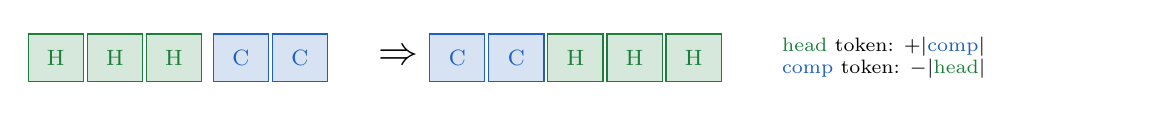
\begin{tikzpicture}[box/.style={draw, minimum width=7mm, minimum height=6mm}, font=\footnotesize]
  \foreach \i in {0,1,2}{\node[box, fill=headc!18, draw=headc] at (\i*0.75,1.3){\head{H}};}
  \foreach \i in {0,1}  {\node[box, fill=compc!18, draw=compc] at (2.35+\i*0.75,1.3){\comp{C}};}
  \node at (4.35,1.3) {\Large$\Rightarrow$};
  \foreach \i in {0,1}  {\node[box, fill=compc!18, draw=compc] at (5.1+\i*0.75,1.3){\comp{C}};}
  \foreach \i in {0,1,2}{\node[box, fill=headc!18, draw=headc] at (6.6+\i*0.75,1.3){\head{H}};}
  \node[anchor=west, font=\scriptsize] at (9.1,1.3)
    {\begin{minipage}{4.4cm}\head{head} token: $+|\comp{\text{comp}}|$\\ \comp{comp} token: $-|\head{\text{head}}|$\end{minipage}};
\end{tikzpicture}
\end{center}

\noindent \code{\_s2\_closer} groups that sum by \textbf{flip type} into four additive pieces. Each is a
(weighted) \textsc{Stab} over the enclosing flips of that type, plus a local head bonus.

\begin{algorithm}[H]
\caption{\textsc{Displacement} --- four additive families}
\begin{algorithmic}[1]
\State $\sop{d\_adv} \gets (+1$ at a verb before an adverb$)\ +\ (-1$ at an adverb$)$ \Comment{purely local swap}
\State $\sop{d\_cp} \gets -\sop{depth}\ +\ \textsc{Where}\big(\sop{isThat},\ \sop{e}-\sop{i}+1,\ 0\big)$ \Comment{clause body $-1$ each; the \emph{that} $+|$clause$|$}
\State $\sop{d\_nprel} \gets \underbrace{(+|\text{RC}|\text{ on the core noun})}_{\text{head bonus}}\ -\ \underbrace{\textsc{Stab}(\text{RC ends, weighted by }|\text{core}|)}_{\text{every token inside a RC}}$
\State $\sop{d\_vp} \gets \underbrace{(+|\text{comp}|\text{ on the verb block})}_{\text{head bonus}}\ -\ \underbrace{\textsc{Stab}(\text{comp ends, weighted by }|\text{head}|)}_{\text{every token inside a VP comp}}$
\State \Return $\sop{d\_adv}+\sop{d\_cp}+\sop{d\_nprel}+\sop{d\_vp}$
\end{algorithmic}
\end{algorithm}

\begin{rulebox}[Read one row of the example]
\emph{chases}$_3$ is the \head{head} of its own VP ($\head{+2}$), but it also sits \emph{inside} the
relative clause (\comp{$-1$} from \code{d\_cp}) and \emph{inside} the NP's relative-clause complement
(\comp{$-1$} from \code{d\_nprel}). Total $\;\head{+2}\comp{-1}\comp{-1}=0$: it never moves.
\end{rulebox}

% ==========================================================================
\section{Stage 3 --- invert and gather}

\begin{algorithm}[H]
\caption{\textsc{Invert} $+$ gather --- apply the permutation}
\begin{algorithmic}[1]
\State $\sop{hfPos} \gets \sop{i} + \sop{disp}$ \Comment{token $i$ wants slot $\sop{hfPos}[i]$}
\State $\sop{src}[j] \gets$ the unique $i$ with $\sop{hfPos}[i]=j$ \Comment{one head: match slot $j$ against \sop{hfPos}}
\State \Return $\textsc{Gather}(\sop{ids},\ \sop{src})$ \Comment{slot $j$ takes the token at $\sop{src}[j]$}
\end{algorithmic}
\end{algorithm}

\noindent Exactly one $i$ matches each $j$ because \sop{hfPos} is a genuine bijection --- that is the
built-in correctness check.

\begin{center}
\tokflow{1.75}
  {0/the, 1/boy, 2/that, 3/chases, 4/the, 5/dog, 6/swims}
  {0/the, 1/the, 2/dog, 3/chases, 4/that, 5/boy, 6/swims}
  {0/0/invc/0, 1/5/headc/{+4}, 2/4/headc/{+2}, 3/3/invc/0, 4/1/compc/{-3}, 5/2/compc/{-3}, 6/6/invc/0}
\end{center}

% ==========================================================================
\section{End-to-end, every number}

\begin{center}\footnotesize
\setlength{\tabcolsep}{5pt}
\begin{tabular}{@{}l|ccccccc@{}}
\toprule
 & the$_0$ & boy$_1$ & that$_2$ & chases$_3$ & the$_4$ & dog$_5$ & swims$_6$\\
\midrule
\code{lc}          & D & N & THAT & V & D & N & V\\
\code{role}        & 0 & 0 & 0 & 2 & 0 & 0 & 1\\
\code{dpFlat}      & 1 & 1 & 2 & 3 & 5 & 5 & 6\\
\code{hasRC}       & 1 & 0 & 0 & 0 & 0 & 0 & 0\\
\midrule
\code{dpfull}      & \flip{5} & 1 & 2 & 3 & 5 & 5 & 6\\
\code{vpe}         & 0 & 1 & 2 & \flip{5} & 4 & 5 & 6\\
\code{rce}         & 0 & 1 & \flip{5} & 3 & 4 & 5 & 6\\
\midrule
\code{e}           & 0 & 1 & \head{5} & 3 & 4 & 5 & 6\\
\code{depth}       & 0 & 0 & 1 & 1 & 1 & 1 & 0\\
\midrule
\code{d\_cp}       & 0 & 0 & $+3$ & $-1$ & $-1$ & $-1$ & 0\\
\code{d\_nprel}    & 0 & $+4$ & $-1$ & $-1$ & $-1$ & $-1$ & 0\\
\code{d\_vp}       & 0 & 0 & 0 & $+2$ & $-1$ & $-1$ & 0\\
\midrule
\code{disp}        & 0 & $+4$ & $+2$ & 0 & $-3$ & $-3$ & 0\\
\code{hfPos}       & 0 & 5 & 4 & 3 & 1 & 2 & 6\\
\code{src}         & 0 & 4 & 5 & 3 & 2 & 1 & 6\\
\bottomrule
\end{tabular}
\end{center}

\noindent Reading \code{src}: slot $1$ takes token $4$ (\emph{the}), slot $2$ takes token $5$ (\emph{dog}), \dots
giving \texttt{the the dog chases that boy swims}.

\begin{keybox}[The whole program in four sentences]
\textbf{(1)} Label each token from itself and two neighbours (\sop{role} decides who flips).
\textbf{(2)} Compute \emph{where} each constituent's complement starts, then \textsc{Gather} its end
from there --- repeating $K$ times, because ends depend on nested ends.
\textbf{(3)} Count enclosing intervals (\textsc{Stab}) to get \sop{depth} and each token's $\pm$ shifts.
\textbf{(4)} Add the shifts to get a target slot, invert, gather.
\end{keybox}

\vfill
\begin{center}\footnotesize\itshape
Every value above is machine-verified against \texttt{\_s2\_closer.hi\_to\_hf} and
\texttt{grammar\_oracle.py} (see \texttt{\_closer\_viz.py}).
\end{center}

\end{document}
